\documentclass[12pt, bibliography=totoc]{scrartcl}
\title{Predicting Blood Pressure from Photoplethysmogram Waveform Data: A Signal Processing and
Machine Learning Approach}
\author{Hugas Jasinskas}
\usepackage{graphicx}
\usepackage{wrapfig}
\usepackage{url}
\usepackage{setspace}
\usepackage{tabto}
\usepackage[export]{adjustbox}
\usepackage{float}
\usepackage[utf8]{inputenc}
\usepackage{csquotes}

\begin{document}

\begin{titlepage}
	\begin{center}
		\vspace*{1cm}
		\begin{figure}[h]
      		\centering
			
\includegraphics[scale=0.6]{Images/hs/hd}
			
\includegraphics[scale=1]{Images/hs/hhn}
			
\includegraphics[scale=0.06]{Images/hs/tmu}
			\label{fig:unis}
		\end{figure}
		
        \vspace*{1cm}
            
        \Huge
        \textbf{Master's Thesis}
            
        \vspace{0.5cm}
        \Large
        Medical Informatics Master
        
        \vspace{0.5cm}
        \Large
        Universität Heidelberg / Hochschule Heilbronn
        
        \vspace{0.5cm}
        \Large
        in Cooperation with Taipei Medical University
        
        \hrulefill
            
        \vspace{1cm}
        
        \Huge
        \textbf{Predicting Blood Pressure from Photoplethysmogram Waveform Data: A Signal Processing and
Machine Learning Approach}
        
    	\end{center}
    
		\vfill
    		\Large
    		\noindent
    		Supervisor: \tab\hspace{-2cm} Prof.\ Dr. Rolf Bendl\\
    		Co-Supervisor: \tab\hspace{-2cm} Prof.\ Dr. Syed Abdul Shabbir\\
    		Submitted by: \tab\hspace{-2cm} Hugas Jasinskas\\
    		Matriculation number: \tab\hspace{-2cm} 202509\\
    		Submitted on: \tab\hspace{-2cm} \today{}\\
    
\end{titlepage}

\newpage

\begin{Huge}
	\centerline{Affidavit}
\end{Huge}

\vspace{2cm}

\begin{Large}

I hereby declare under oath that I have independently prepared the present work without using sources other than those indicated; any thoughts taken directly or indirectly from external sources (including electronic sources) are identified as such.

The work has not been submitted to any examination authority, either domestic or foreign, in the same or similar form, and has not been published.

\end{Large}

\vfill

\rule{4cm}{0.5mm} \tab \rule{4cm}{0.5mm}

Place, Date \tab Signature

\newpage

\tableofcontents

\newpage
\onehalfspacing

\section{Abstract}\label{sec:abstract}


\section{Introduction}
\label{sec:introduction}
\subsection{Subject and Motivation}
\label{subsec:subject_motivation}

Cardiovascular diseases (CVDs) are the leading cause of death worldwide, according to WHO publishing statistics~\cite{organizationWorldHealthStatistics2023}.
One of the main factors contributing to CVDs is Hypertension.
It is the leading risk factor for mortality, and is ranked third as a cause of disability-adjusted life-years~\cite{ezzatiSelectedMajorRisk2002}.
Currently, there is a significant need for continuous blood pressure (BP) monitoring due to various factors.
Primarily, while hypertension is a manageable condition, the availability of accurate high BP detection remains scarce, especially in low-resource environments~\cite{burtPrevalenceHypertensionUS1995}.
Additionally, blood pressure (BP) is subject to rapid fluctuations influenced by various factors, including stress, emotions, dietary intake, physical activity, and medication usage~\cite{poonCufflessNoninvasiveMeasurements2005}.
Continuous monitoring of blood pressure, rather than relying on isolated measurements, plays a vital role in the early detection and treatment of hypertension~\cite{el-hajjDeepLearningModels2021}.

The current accurate methods for measuring BP continuously are either invasive or involving a cuff-mechanism.
Catheterization is internationally recognized as the \enquote{gold standard} for obtaining the most accurate measurement of continuous blood pressure~\cite{sharmaCuffLessContinuousBlood2017}.
However, due to its invasive nature and limited applicability to hospital settings, this method requires medical intervention, which renders it inconvenient for everyday use.

While cuff-based devices are commonly utilized for this objective, it is worth noting that around 30\% of home blood pressure monitors are found to be inaccurate, rendering continuous measurement unfeasible~\cite{leungHypertensionCanada20162016, seboBloodPressureMeasurements2014}.
Moreover, this approach relies on the individual consciously and intentionally engaging in manual blood pressure monitoring, which poses limitations and might be often overlooked.

An ideal technology for measuring blood pressure should have the following attributes: non-invasiveness, cuffless operation, optical functionality, wearable design, and cost-effectiveness~\cite{el-hajjDeepLearningModels2021}.
One approach satisfying these requirements is the estimation of BP from a single measurement PPG sensor.
This approach, using two modes, reflectance and transmission, has gained an increasing amount of attention in the literature due its simplicity, and ability to provide continuous and cuffless measurement~\cite{el-hajjDeepLearningModels2021}.
Typically, the photoplethysmography (PPG) technique has been traditionally employed in healthcare settings to measure heart rate~\cite{reyesWirelessPhotoplethysmographicDevice2012} and blood oxygen saturation using a pulse oximeter~\cite{yoonMultipleDiagnosisBased2002}.

Nevertheless, establishing a straightforward, distinct, and continuous relationship between these characteristics and blood pressure (BP) has proven to be challenging.
To address this, the approach heavily depends on signal pre-processing techniques, extracting PPG features, and utilizing machine learning (ML) algorithms to estimate BP based on these features~\cite{el-hajjDeepLearningModels2021}.
A recent scoping review by Knight et al.\ concluded that PPG can be successfully used to continuously measure BP, by evaluating latest publications and finding over 80\% accuracy in detecting hypertension~\cite{knightAccuracyWearablePhotoplethysmography2022}.

This study examines the current methods and aims to develop efficient approaches for the continuous and accurate measurement of blood pressure using PPG and addresses the following research questions:

\begin{enumerate}
    \item \textbf{What is the relationship between PPG data and blood pressure among Intensive Care Unit (ICU) patients?}

    \item \textbf{Can PPG-based data be used to estimate blood pressure accurately?}

\end{enumerate}

\subsection{Tasks and Objectives}
\label{subsec:tasks_objectives}

The tasks of the thesis are as follows:

\begin{enumerate}
    \item Signal Processing: to find an optimal data fetching and filtering approach from available MIMIC Databases.
    \item Likewise, to create a consistent algorithm for key feature extraction.
    \item Machine Learning: to develop a model based on the resulting features from Signal Processing, to reliably predict BP from PPG\@.
\end{enumerate}

\subsection{Structure of the Thesis}
\label{subsec:structure}

This thesis is organized as follows:

In Chapter~\ref{sec:background}, the foundations of the used terms and prerequisites for the methods are explained.
For example, in~\ref{subsec:med_background}, the terms \enquote{Blood Pressure} (\ref{subsubsec:bp}) and \enquote{Photoplethysmography} (\ref{subsubsec:ppg}) are discussed.
Furthermore, the general structure of MIMIC databases is explained (\ref{subsubsec:mimic}).
In addition, the essential information about the Computing part of this research is provided (\ref{subsec:computing_background}).

In Chapter~\ref{sec:methods}, the methodology is explained.

Chapter~\ref{sec:results} presents the results.

The focus of Chapters~\ref{sec:discussion} and~\ref{sec:conclusion} is on summarizing the work.
Here, both the future prospects for this research field and the next steps in relation to broader scope projects are presented.

\section{Theoretical Background}
\label{sec:background}
\subsection{Medical Background}
\label{subsec:med_background}

\subsubsection{Blood Pressure}
\label{subsubsec:bp}

% general BP
Blood pressure (BP) is a physiological measure of the force exerted by circulating blood against the walls of the arteries~\cite{WhatBloodPressure2019}.
It is highly dependent on blood flow, which refers to the movement of blood through a vessel, tissue, or organ.
Blood circulation begins with the contraction of the heart's ventricles.
This action generates a type of hydrostatic pressure, which is the force exerted by a fluid due to gravitational pull, typically against the walls of the container that confines it.

BP is a type of hydrostatic pressure, representing the force exerted by blood on the walls of blood vessels or the heart's chambers.
While it can be assessed in various body regions, the term \enquote{blood pressure} without specific qualifiers commonly refers to systemic arterial BP\@.
This denotes the pressure of blood within the arteries of the systemic circulation.
In clinical settings, this pressure is measured in millimeters of mercury (mmHg) and is typically acquired using the brachial artery in the arm~\cite{betts20BloodFlow2022}.

% measuring significance
Measuring BP is crucial for assessing cardiovascular health and identifying potential risks.
It allows for the early detection of conditions like hypertension and hypotension, enabling timely interventions to prevent serious cardiovascular events~\cite{naylorArterialCathetersEarly2020}.
BP serves as a key indicator of the risk for heart attacks, strokes, and heart failure, guiding preventive measures and treatment strategies~\cite{ettehadBloodPressureLowering2016}.

\vspace{0.2cm}
\textit{Various Types of Measurement}
\vspace{0.2cm}

% cuff BP measuring
One of the most common BP measurement methods is one using a sphygmomanometer (see manual~\ref{fig:sphyg} and automatic~\ref{fig:auto_sphyg} devices), also known as non-invasive blood pressure (NIBP), is typically recorded as numeric values at specific time intervals.
The process involves inflating the cuff to temporarily stop blood flow and then gradually releasing the pressure to detect the sounds associated with the flow of blood through the brachial artery.
Manually, the measurement entails one individual conducting the procedure on another, typically involving a healthcare professional administering the assessment to a patient.
Conversely, automatic measurement allows the patient to independently measure their blood pressure without external assistance.
Both approaches yield comparable measurements of the same nature.
The two primary values obtained are systolic pressure (maximum pressure during heartbeats) and diastolic pressure (minimum pressure between heartbeats).
During the process of cuff inflation and deflation, each heartbeat generates characteristic sounds (Korotkoff sounds) that are detected by a stethoscope placed over the brachial artery.
Systolic pressure is recorded when the first tapping sounds are heard, and diastolic pressure is recorded when the sounds disappear or change character.
This beat-to-beat approach provides information about individual fluctuations in blood pressure~\cite{betts20BloodFlow2022}.

\begin{figure}[h]
    \centering
    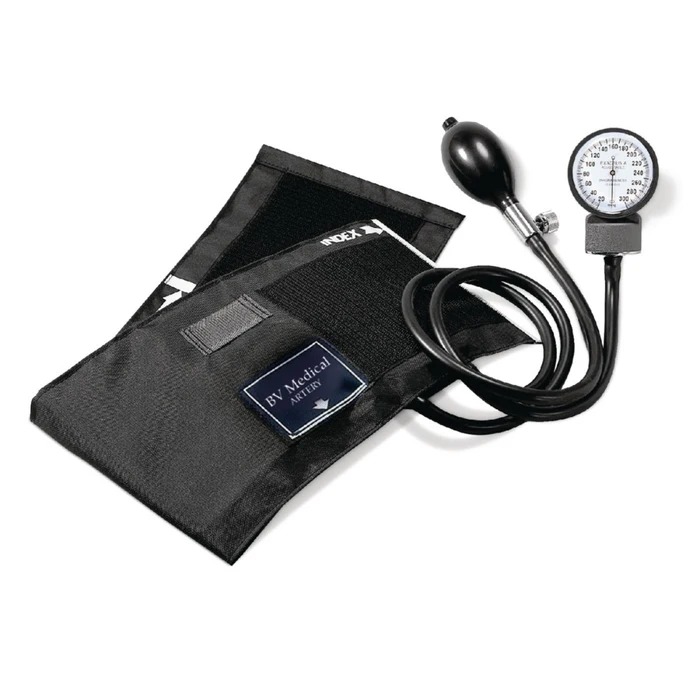
\includegraphics[scale=0.2]{images/abp/sphyg}
    \caption{Standard Sphygmanometer \cite{StandardSphygmomanometer}}
    \label{fig:sphyg}
    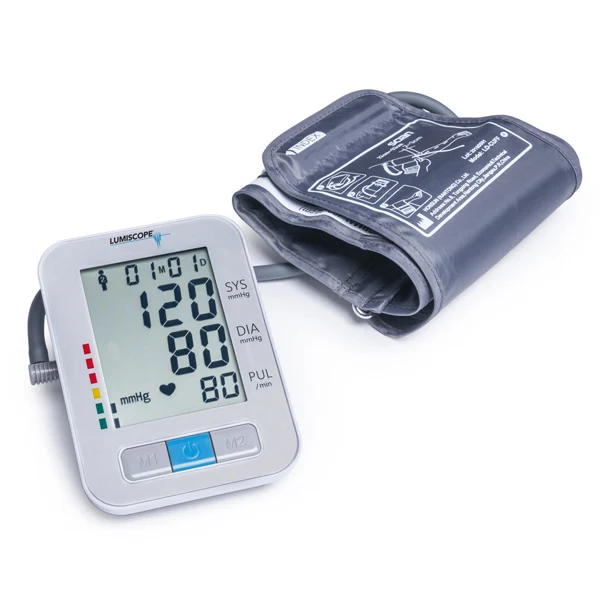
\includegraphics[scale=0.2]{images/abp/auto_sphyg}
    \caption{Automatic Digital Sphygmanometer \cite{AutomaticDigitalBlood}}
    \label{fig:auto_sphyg}
\end{figure}

Although measuring blood pressure with a cuff using a sphygmomanometer is widely adopted as a common and convenient method, it is not without its constraints.
Studies, such as those by Leung et al.\ and Sebo et al.\ , have highlighted the inability of home blood pressure monitoring devices to consistently and accurately detect hypertension~\cite{leungHypertensionCanada20162016, seboBloodPressureMeasurements2014}.
Furthermore, a significant limitation lies in its inability to provide continuous and consistent monitoring, necessitating patients to actively remember and engage in the effort to measure their blood pressure.
This intermittent approach using a cuff provides valuable insights into systolic and diastolic pressures at specific time intervals, but it may not capture the nuanced changes that occur between measurements.
To address the need for continuous monitoring, other methods, such as arterial catheterization, are employed.

% arterial BP
Arterial catheterization (illustrated in Figure~\ref{fig:catheter}) is commonly employed in critical patient care, serving dual purposes: continuous blood pressure monitoring and obtaining frequent blood gas measurements.
Typically conducted at bedside, the procedure utilizes percutaneous methods like the Seldinger technique to cannulate arteries~\cite{clarkArterialCatheterization1992}.
The resulting arterial blood pressure (ABP) is a dynamic parameter that can change with each heartbeat, and it is typically represented as a waveform rather than a single numeric value.
The ABP waveform consists of two main components: systolic pressure and diastolic pressure.
Such continuous monitoring of ABP is usually done in clinical settings, using an arterial line connected to a pressure transducer.
The resulting waveform is displayed on a monitor in real-time.
However, for ease of interpretation and documentation, numeric values are commonly extracted from the waveform at specific time intervals~\cite{hillImputationContinuousArterial2021}.

\begin{figure}[h]
    \centering
    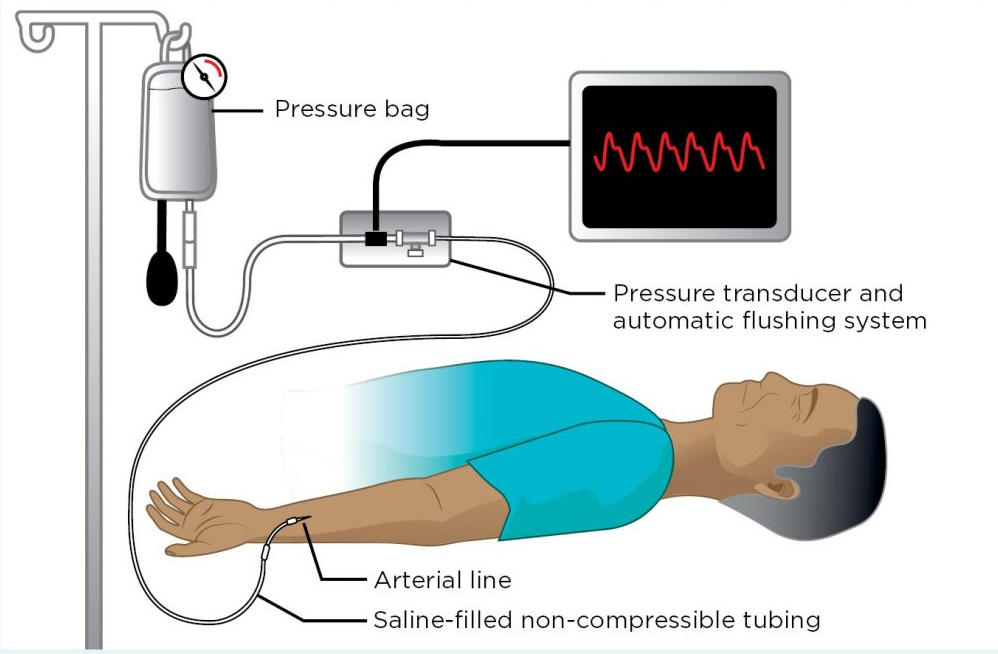
\includegraphics[scale=0.4]{images/abp/catheter}
    \caption{Arterial Catheterization and Stationary BP Monitoring~\cite{contributorEssentialCriticalCare2021}}
    \label{fig:catheter}
\end{figure}

In situations where high temporal resolution is crucial, ABP can be recorded beat-to-beat, providing a value for each heartbeat.
This is particularly important in situations where rapid changes in blood pressure need to be closely monitored, such as during certain medical procedures or in critically ill patients~\cite{lehmanMethodsBloodPressure2013}.

For routine monitoring and documentation, numeric values are often averaged over a specific time interval, such as every 1, 5, or 15 minutes.
This averaged value may be reported as the mean arterial pressure (MAP), which is a weighted average of the systolic and diastolic pressures over a cardiac cycle~\cite{demersPhysiologyMeanArterial2024}
Some monitoring systems may also provide systolic and diastolic blood pressure readings at regular intervals.

Alternative approaches for measuring BP have emerged over the past years.
Volume clamping~\cite{kimBallistocardiogramBasedApproachCuffless2018} and tonometry~\cite{imholzFifteenYearsExperience1998} are some of the other methods.
These non-invasive techniques offer continuous monitoring of blood pressure values.
Volume clamping, which involves the use of a small finger cuff and a PPG sensor, is one method for continuous blood pressure measurement.
Tonometry, on the other hand, is a cuffless approach that utilizes a manometer-tipped probe pressed directly on an artery.
The volume clamping approach allows for instantaneous and prolonged blood pressure measurement.
However, it is associated with high costs and still necessitates the use of a cuff, which can be inconvenient and uncomfortable.
Conversely, the tonometry method is sensitive to movement of the arm and probe, making it challenging to maintain accuracy in practical applications.
Additionally, constant calibration with a cuff blood pressure device is required~\cite{peterReviewMethodsNoninvasive2014}.

\vspace{0.2cm}

In conclusion, blood pressure serves as a critical physiological measure, representing the force exerted by blood on the walls of blood vessels.
The conventional method of measuring blood pressure with a cuff and sphygmomanometer provides valuable insights into systolic and diastolic pressures but is limited by its intermittent nature.
To address the need for continuous monitoring, arterial catheterization is commonly employed in critical care, offering real-time data through a dynamic waveform.
Alternative non-invasive approaches like volume clamping and tonometry aim to provide continuous blood pressure monitoring, but they come with their own challenges and considerations.
As technology advances, these methods contribute to a comprehensive understanding of blood pressure dynamics, facilitating improved patient care and risk assessment.

\subsubsection{Photoplethysmography}
\label{subsubsec:ppg}

% meaning and basic information
Photoplethysmography (PPG) is an optical measurement technique designed to identify changes in blood volume within the microvascular bed of tissue~\cite{challonerPhotoelectricPlethysmographMeasurement1974}.
Its clinical application is extensive, as the technology is integrated into commercially available medical devices, including pulse oximeters, vascular diagnostics, and digital beat-to-beat blood pressure measurement systems.
The fundamental structure of PPG technology is straightforward, requiring only a few opto-electronic components: a light source for tissue illumination, usually a light-emitting diode (LED) and a photodiode (PD) to gauge slight variations in light intensity correlated with changes in perfusion in the catchment volume.

% history and origins
\vspace{0.2cm}
\textit{History}
\vspace{0.2cm}

One of the first mentioned instances on the use of PPG were recorded in 1936 by Molitor and Kniazuk~\cite{molitorNewBloodlessMethod1936}.
They outlined comparable devices employed for tracking alterations in blood volume in the rabbit ear under conditions of venous occlusion and the administration of vasoactive drugs.
A pioneer who helped establish the PPG technique was Alrick Hertzman~\cite{hertzmanPhotoelectricPlethysmographyFingers1937}.
In his 1937 paper, Hertzman coined the term \enquote{Photoelectric Plethysmograph} etymologically meaning:
photo - \enquote{light}, plethora - \enquote{exess of body fluid, blood}, graph - \enquote{something written}.
He detailed the application of a reflection mode system to assess alterations in blood volume within the fingers, particularly during the Valsalva maneuver~\cite{srivastavValsalvaManeuver2024}, exercise, and exposure to cold.
This contribution not only demonstrated the versatility of the technique but also underscored its potential clinical relevance.

Hertzman and Spealman~\cite{hertzmanPhotoelectricPlethysmographyFingers1937} outlined two crucial features of the PPG pulse waveform.
They categorized the pulse appearance into two phases: the anacrotic phase representing the ascending edge of the pulse, and the catacrotic phase representing the descending edge of the pulse.
The initial phase primarily corresponds to systole, while the subsequent phase relates to diastole and wave reflections from the periphery.
In individuals with healthy compliant arteries, a dicrotic notch is commonly observed during the catacrotic phase.

In the late 1970s, there arose a renewed interest in the PPG technology, driven by the demand for compact, dependable, cost-effective, and user-friendly noninvasive cardiovascular assessment techniques~\cite{yoshiyaSpectrophotometricMonitoringArterial1980}.
The progress in opto-electronics and clinical instrumentation has played a significant role in advancing PPG technology.
Semiconductor advancements, particularly in LEDs, photodiodes, and phototransistors, have brought about substantial improvements in the size, sensitivity, reliability, and reproducibility of PPG probe design.
A significant leap in the clinical application of PPG-based technology occurred with the introduction of the pulse oximeter~\cite{aoyagiPulseOximetryIts2002}.
This device revolutionized non-invasive monitoring of patients' arterial oxygen saturation, marking a major advancement in the field.

Other emerging technologies encompass PPG imaging technology, telemedicine, and remote monitoring.
In 2005, Wieringa et al.\ detailed a contactless multiple-wavelength PPG imaging system designed primarily for remotely imaging the distribution of arterial oxygen saturation (SpO2) within tissue~\cite{wieringaContactlessMultipleWavelength2005}.
The system captures movies of two-dimensional matrix spatially resolved PPG signals at different wavelengths during respiratory changes.
PPG was found to have substantial potential in telemedicine, particularly for remote/home health monitoring of patients.
Miniaturization, user-friendliness, and robustness stand as pivotal design criteria for such systems.
This is exemplified by finger ring-based PPG sensors for monitoring beat-to-beat pulsations (\cite{rheeArtifactresistantPowerefficientDesign2001}, ~\cite{zhengRingtypeDeviceNoninvasive2003}).

Most PPG devices these days either use the transmissive or reflective operating modes (illustrated in Figure~\ref{fig:reflection}).
Currently, the prevalent method is the transmissive mode, chosen for its notable accuracy and stability~\cite{leeReflectancePulseOximetry2016}.
However, there is a growing interest in reflective-mode PPG due to its elimination of the need for a thin measurement site.
This method proves versatile, applicable to various sites such as the feet, forehead, chest, and wrists.
Especially when the wrist serves as the designated measurement site, PPG sensors can be conveniently employed in the form of a band or watch.

\begin{figure}[h]
    \centering
    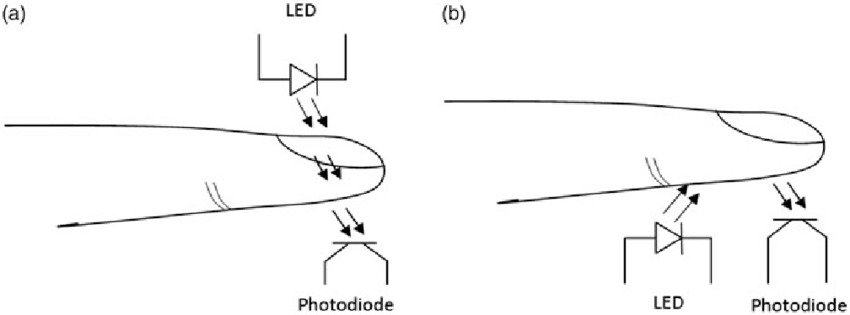
\includegraphics[scale=0.4]{images/ppg/reflection}
    \caption{PPG Transmission (a) and Reflection (b) operating modes \cite{mohanSpotMeasurementHeart2016}}
    \label{fig:reflection}
\end{figure}

% how does it work
\vspace{0.2cm}
\textit{Working Principle}
\vspace{0.2cm}

The PPG signal consists of pulsate (AC) and superimposed (DC) components (see Figure~\ref{fig:acdc}).
The AC component originates from variations in blood volume associated with heartbeats,
while the DC component is influenced by factors such as respiration, sympathetic nervous system activity, and temperature regulation~\cite{allenPhotoplethysmographyItsApplication2007a}.
The AC component specifically illustrates changes in blood volume during phasic cardiac activity, representing both the systolic and diastolic phases.
The systolic phase, also known as the \enquote{rise time} initiates with a valley and concludes at the pulse wave systolic peak.
The pulse wave concludes with another valley at the end of the diastolic phase~\cite{weisslerSystolicTimeIntervals1968}.
In most PPG waveform analyses including this one, the AC component in the form of a waveform signal is used.

\begin{figure}[h]
    \centering
    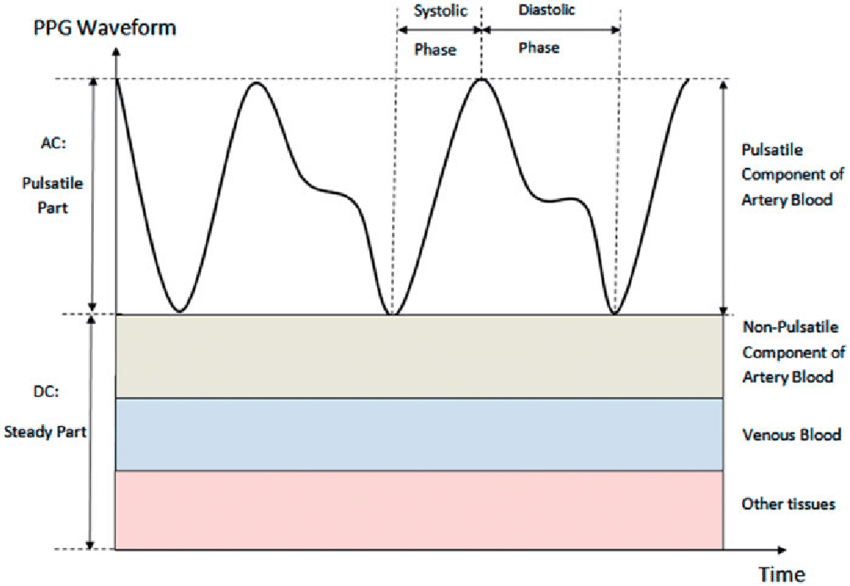
\includegraphics[scale=0.5]{images/ppg/ac+dc}
    \caption{AC and DC components of the PPG signal \cite{mohanSpotMeasurementHeart2016}}
    \label{fig:acdc}
\end{figure}

% main and potential use cases
\vspace{0.2cm}
\textit{Use Cases}
\vspace{0.2cm}

PPG finds diverse applications in clinical settings, covering physiological monitoring (such as blood oxygen saturation and heart rate), vascular assessment (including arterial disease, aging and tissue viability), and autonomic function evaluations (such as thermoregulation, heart rate and other assessments of cardiovascular variability)~\cite{allenPhotoplethysmographyItsApplication2007a}.
Furthermore, the popularity of PPG technology as an alternative for monitoring heart rate has risen recently, primarily attributed to its ease of use, user-friendly wearing comfort, and cost-effectiveness~\cite{sviridovaHumanPhotoplethysmogramNew2015}.
Nowadays, almost every wearable devices uses the PPG technology to track the user's heart rate and other extractable vital parameters~\cite{castanedaReviewWearablePhotoplethysmography2018}.
PPG sensors in mobile and wearable devices typically feature red, green, or both light-emitting diodes.
Most devices incorporate a green-light PPG sensor for continuous heart rate monitoring during daily activities.
Some devices also include red-light PPG sensors, which are effective for measuring heart rate when a person is stationary, providing insights into hydration, muscle saturation, and total hemoglobin.
While red-light PPG can penetrate tissue layers more deeply using near-infrared spectroscopy, it is susceptible to disturbance from ambient light.
In contrast, green light, being less absorbed by the skin, minimizes the impact of ambient light noise on the heart rate signal.
As a result, wearable devices commonly utilize green light rather than red-light PPG~\cite{ponnadaTechnologicalConsiderationsSensorassisted2019}.
Different types of devices implement the PPG technology.
It can be found in pulse oximeters, smartphones, smartwatches and other wearable devices (examples in Figure~\ref{fig:ppg-devices}).

\begin{figure}[h]
    \centering
    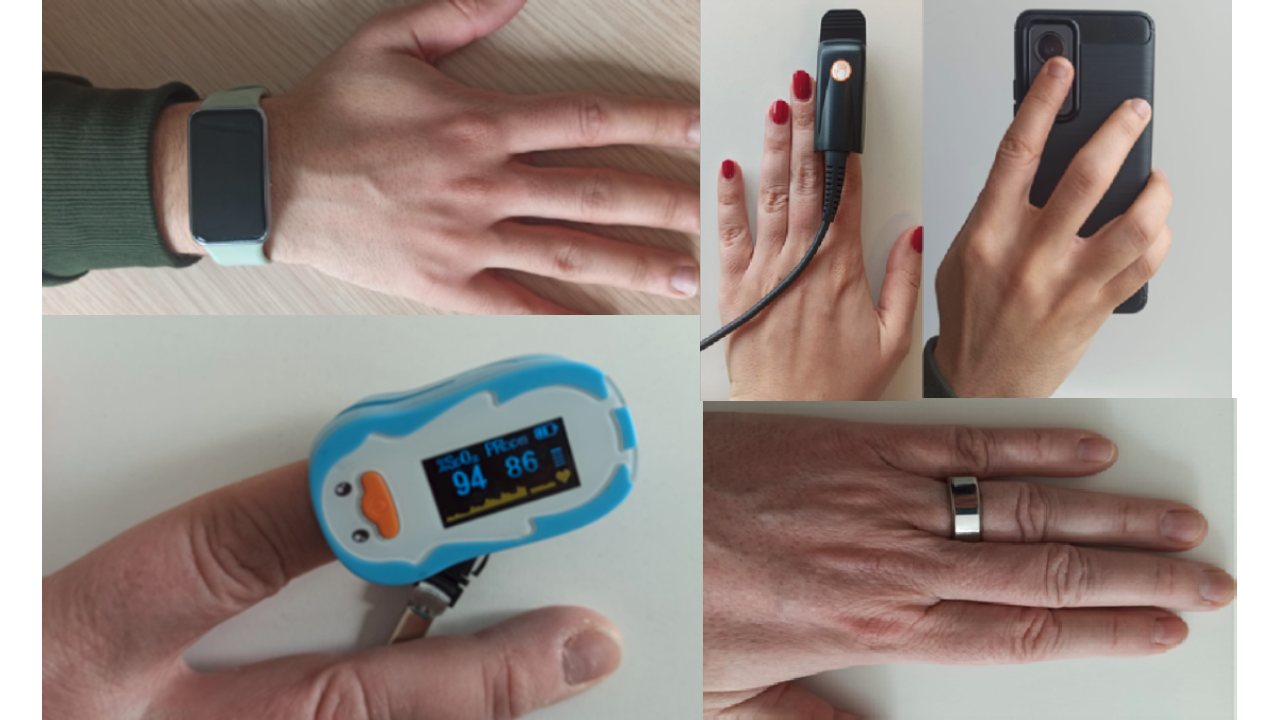
\includegraphics[scale=0.35]{images/ppg/ppg-devices}
    \caption{AC and DC components of the PPG signal \cite{zanelliPotentialAIBased2023}}
    \label{fig:ppg-devices}
\end{figure}

% Conclusion parahraph
\vspace{0.2cm}

In conclusion, the PPG is an optical sensor, consisting of an LED paired with a PD, hence it is simple, inexpensive and can be easily build into a wearable device.
The PPG waveform can be obtained using two modes, reflectance and transmission.
This waveform corresponds to the blood volume in blood vessels.
Traditionally employed in healthcare for heart rate and blood oxygen saturation measurements, particularly with pulse oximeters, the PPG plays a pivotal role~\cite{allenPhotoplethysmographyItsApplication2007a}.

% outlook to SP and ML
Additionally, peripheral volumetric changes exhibit correlation with BP~\cite{langewoutersPressurediameterRelationshipsSegments1986}.
Utilizing characteristic PPG features, ML functions can estimate Systolic BP (SBP) and Diastolic BP (DBP).
However, establishing a simple, clear, and continuous relationship between these features and BP remains elusive.
This method heavily relies on signal pre-processing, feature extraction, and the application of ML algorithms for BP estimation based on these features.

\subsubsection{MIMIC Databases}
\label{subsubsec:mimic}

Patient records and documentation are crucial for maintaining a comprehensive overview of medical history, aiding in accurate diagnosis, treatment planning, and ensuring continuity of care.
They also serve as legal documents, providing evidence of the care provided and facilitating communication among healthcare professionals.
Collecting digital data during routine clinical practice has become widespread across hospitals.
Over time, a pattern has emerged in the collection and storage of patient data for subsequent utilization in future research endeavors.

% History and Origin
\vspace{0.2cm}
\textit{Origin}
\vspace{0.2cm}

In 1996, two researchers at the Massachusetts Institute of Technology, George B. Moody and Roger G. Mark, introduced the Multiparameter Intelligent Monitoring in Intensive Care (MIMIC) Database (DB).
The DB was derived from patient monitors in the medical, surgical, and cardiac ICUs of Boston’s Beth Israel Hospital~\cite{moodyDatabaseSupportDevelopment1996}.
The first instance of the DB included 100 patient records, each typically containing between 24 and 48 hours of continuous recorded data.
The second version of the DB (MIMIC-II) was introduced in 2011 boasting a notably larger sample size and a wider scope of information sourced entirely from diverse digital information systems~\cite{saeedMultiparameterIntelligentMonitoring2011}.
MIMIC-III~\cite{johnsonMIMICIIIFreelyAccessible2016} was finalized in 2016, marking a significant expansion from MIMIC-II, with data available from over 40,000 patients.
The fourth and latest MIMIC DB was publicly released in 2023 spanning a decade of admissions from 2008 to 2019.
MIMIC-IV was announced to enhance the realm of publicly accessible critical care datasets, by integrating precise digital sources like the electronic medicine administration record and featuring a modular structure enabling seamless integration with external departments and diverse data modalities~\cite{johnsonMIMICIVFreelyAccessible2023}.
The diagram in Figure~\ref{fig:mimic_workflow} depicts the component interaction for data and information delivery to the publicly available DB\@.

\begin{figure}[h]
    \centering
    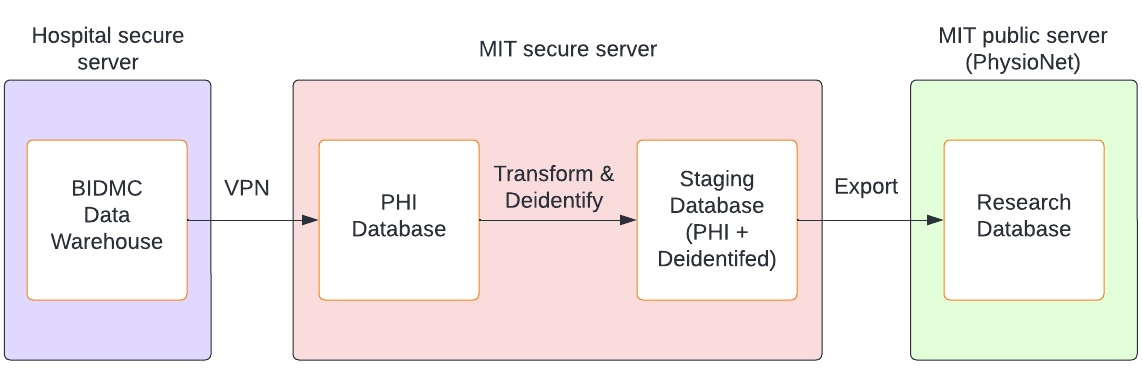
\includegraphics[scale=0.6]{images/mimic/mimic_workflow}
    \caption{Workflow between Beth Israel Deaconess Medical Center (BIDMC), Protected Health Information (PHI) DB ~\cite{charltonMIMICWFDBTutorials2022}}
    \label{fig:mimic_workflow}
\end{figure}

% Structure of MIMIC DB
\vspace{0.2cm}
\textit{Structure}
\vspace{0.2cm}

Both the MIMIC-III and MIMIC-IV DBs are cited and employed in this investigation, exhibiting comparable structures (depicted in Figure~\ref{fig:mimic_structure}), encompassing diverse data categories.
However, the primary emphasis of this inquiry lies in the Waveform Section of the DB (highlighted by a red rectangle in Figure~\ref{fig:mimic_structure}).
The waveform DB comprises individual records, each representing a patient's ICU stay and stored in a distinct subdirectory.
These records lack specific date or time data to ensure patient anonymity, relying instead on elapsed time from the record's start.
Supplemented by surrogate date and time information for cross-referencing with other DB modules.
Waveforms denote regularly sampled, high-resolution measurements stored in a signal specific numerical format.
To optimize storage and processing, these waveforms are segmented into intervals, maintaining continuous sampling within each segment despite potential signal unavailability throughout a patient's ICU stay.

\begin{figure}[h]
    \centering
    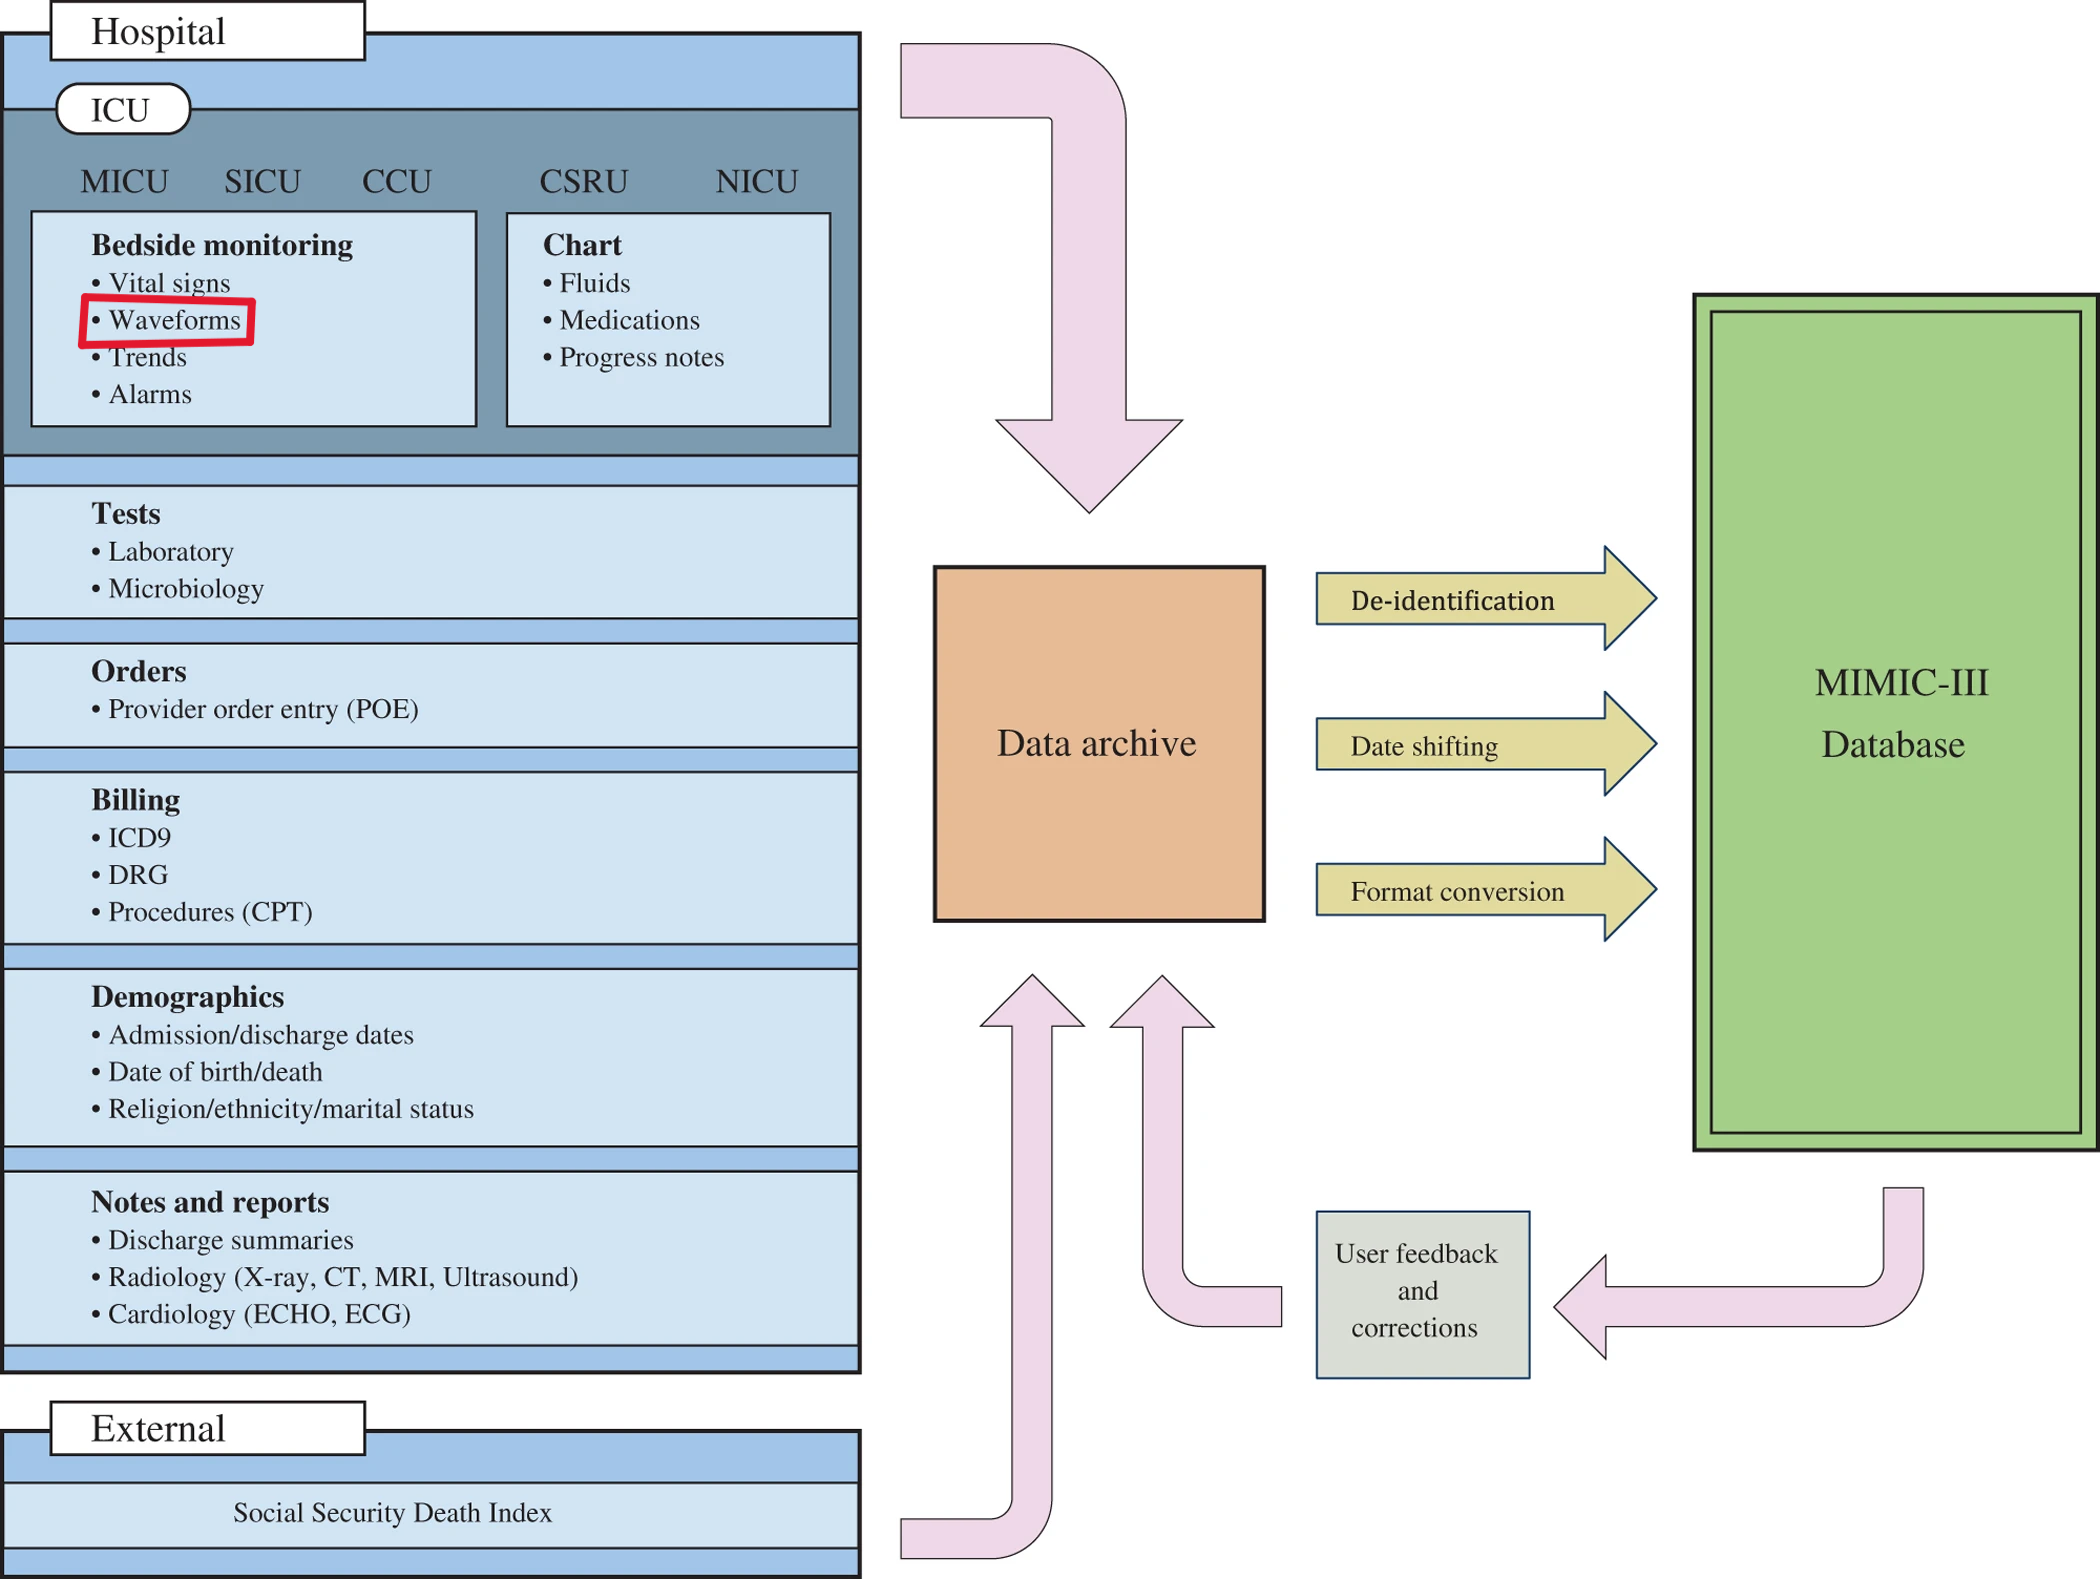
\includegraphics[scale=0.3]{images/mimic/mimic_structure}
    \caption{General Structure of the MIMIC-III DB~\cite{johnsonMIMICIIIFreelyAccessible2016}}
    \label{fig:mimic_structure}
\end{figure}

The Waveform data from both the MIMIC-III and MIMIC-IV DBs is publicly available on the Physionet internet website~\cite{moodyMIMICIIIWaveformDatabase2017, moodyMIMICIVWaveformDatabase}.
In both DBs recorded waveforms typically encompass one or more electrocardiogram(ECG) signals, often feature continuous ABP waveforms and fingertip PPG signals.
Numeric data typically includes heart and respiration rates, SpO2, and systolic, mean, and diastolic blood pressure, among other metrics when accessible.
Recording durations also vary, with most lasting a few days, although some are shorter and other might even extend over several weeks.
Both projects consist of two types of data: waveform data, comprising high-resolution, regularly sampled time series obtained directly from measuring devices, and numeric data, including digitally derived values or irregularly sampled data (like NIBP).

% Differences MIMIC3 and MIMIC4
\vspace{0.2cm}
\textit{Differences and Similarities between MIMIC-III and MIMIC-IV}
\vspace{0.2cm}

In MIMIC-III, waveforms were collected in a largely automated manner from selected adult and neonatal ICUs, resulting in a random sample of patients.
The data archiving process was not continuous, and the recorded waveforms and numerics varied based on ICU staff choices.
The individual patient consent waived due to de-identification.
On the other hand, MIMIC-IV collected data from ICUs where bedside monitors were linked to a local area network, allowing continuous monitoring and data transfer to a proprietary relational DB.
Data was stored for several weeks before being retrieved and archived daily.
The de-identification process for MIMIC-IV followed the same method as MIMIC-III, removing or replacing protected health information with non-identifying information.

Both the MIMIC-III and MIMIC-IV DBs encompass waveform and numeric datasets sourced from ICUs.
While both datasets feature detailed waveform records and numerical values, their storage and acquisition methods differ.
MIMIC-III organizes its records within a directory structure with segmented waveform data, while MIMIC-IV adopts WFDB format for waveforms and compressed CSV files for numerics.
However, MIMIC-IV incorporates enhancements like automated record partitioning and optimized storage formats to enhance data management efficiency.

% Conclusion parahraph
\vspace{0.2cm}

Clinical Research DBs such as MIMIC play a pivotal role in facilitating global access to critical patient data, thereby supporting scientific endeavors across various medical domains.
By ensuring the anonymity and de-identification of patient information, these DBs uphold stringent standards of data privacy and ethics, thereby avoiding any infringement upon patient rights or privacy regulations.
Such DBs serve as invaluable resources for conducting comprehensive studies spanning diverse medical disciplines, including but not limited to the detection and treatment of various cancers, cardiovascular diseases, and even neonatal care in stationary settings.
Their expansive datasets offer researchers an extensive pool of information to draw insights from, ultimately advancing the overall understanding and management of complex medical conditions.

\subsection{Computing Background}
\label{subsec:computing_background}

\subsubsection{Signal Processing}
\label{subsubsec:signal_processing}

This section explores various techniques and methods employed in the analysis of PPG signals and their correlation to BP measurements.
PPG-based BP estimation has emerged as a promising non-invasive approach, utilizing waveform observations from signals like PPG signals from different anatomical sites or their combination with ECG signals.
This section delves into the diverse methodologies and algorithms utilized for processing PPG signals to derive meaningful insights into BP dynamics.

% What are the methods of signal processing for reading PPG?
% Approaches for processing the given PPG data in correlation to BP
\vspace{0.2cm}
\textit{PPG Signal Processing Methods}
\vspace{0.2cm}

% PTT
Previous research has documented an inverse relationship BP and pulse transit time (PTT)~\cite{mukkamalaUbiquitousBloodPressure2015}.
Extensive investigation over past decades has focused on the PTT-based approach, revealing growing support for its potential in offering non-invasive BP measurements without the need for cuffs.
PTT refers to the delay in time for the pressure waveform to traverse between two arterial locations (see Figure~\ref{fig:ptt}).
It can be calculated as the time difference between proximal and distal waveforms indicative of the arterial pulse.
\begin{figure}[h]
    \centering
    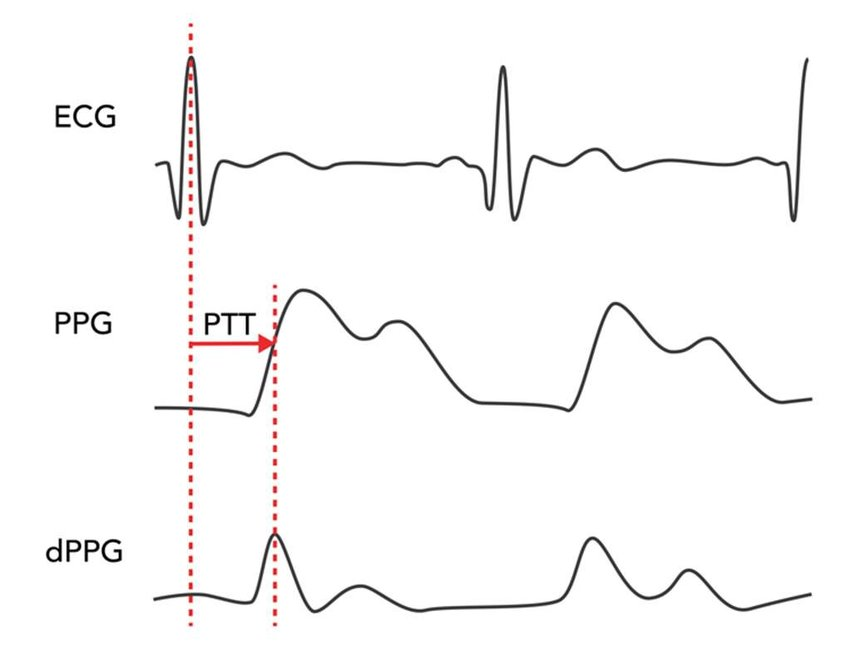
\includegraphics[scale=0.4]{images/sp/ptt}
    \caption{Calculation of PTT from ECG, PPG and first PPG derivative waveforms~\cite{luiNovelCalibrationProcedure2018}}
    \label{fig:ptt}
\end{figure}

% PAT
Pulse arrival time (PAT) represents another widely employed technique~\cite{sharmaCuffLessContinuousBlood2017}.
It is defined as the time that takes the pulse wave to travel from the heart to a peripheral site e.g.\ finger, toe, etc.
It denotes the temporal discrepancy between the R-peak of the ECG signal and the peak of the PPG signal, measured within the same cardiac cycle (see Figure~\ref{fig:pat}).
Both PTT and PAT require simultaneous measurement at two different sites on the body, hence two measurement sensors (ECG and PPG) are needed for recording the signals in order to estimate these parameters.
\begin{figure}[h]
    \centering
    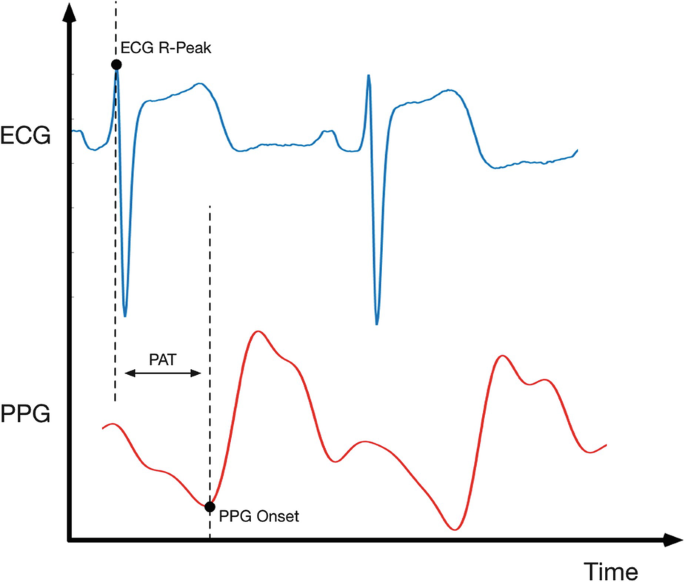
\includegraphics[scale=0.4]{images/sp/pat}
    \caption{Calculation of PAT from ECG and PPG waveforms~\cite{dhillonPulseArrivalTime2019}}
    \label{fig:pat}
\end{figure}

% PWV
Pulse wave velocity (PWV) is another alternative method for estimating BP~\cite{mccombieAdaptiveBloodPressure2006}.
PWV determines the speed of the pulse wave by utilizing two PPG sensors positioned along the same arterial branch, separated by a known distance (see Figure~\ref{fig:pww}), portrayed by the following formula
\begin{math}
    PWW = \frac{D}{PTT}
\end{math}
where D is the distance between two known body parts.

\begin{figure}
    \begin{minipage}[c]{0.5\textwidth}
        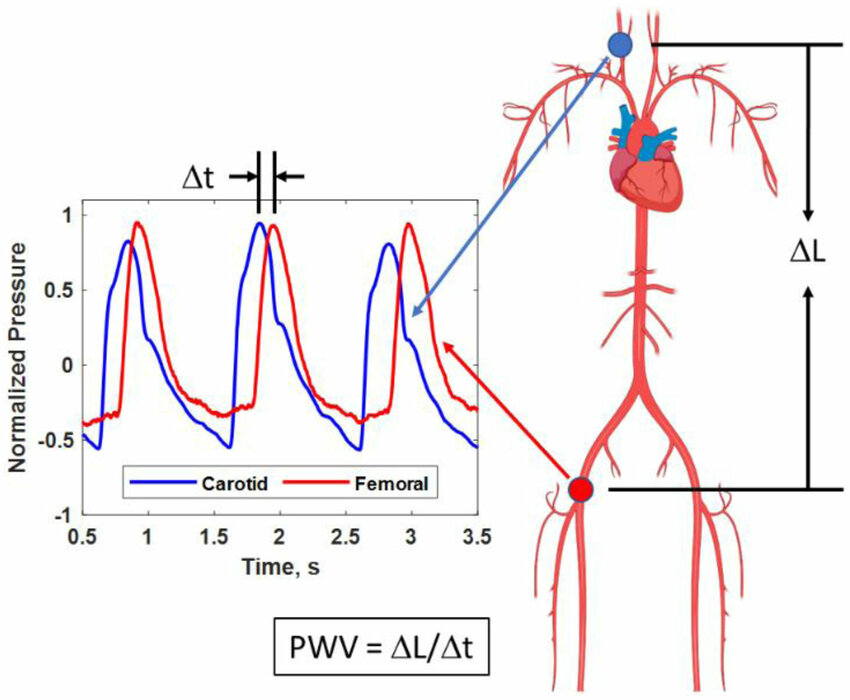
\includegraphics[width=\textwidth]{images/sp/pww}
    \end{minipage}\hfill
    \begin{minipage}[c]{0.5\textwidth}
        \captionsetup{format=plain, justification=centering}
        \caption{Calculation of PWW from two PPG signals at different body parts~\cite{urbanUnderstandingArterialBiomechanics2023}}
        \label{fig:pww}
    \end{minipage}
\end{figure}

% summarize PTT,PAT,PWV
Estimating BP through PTT, PAT, or PWV parameters involves mathematical models, but implementing these models faces challenges, and none of these techniques has become a reliable clinical tool for BP measurement.
Challenges include the need for synchronized sensors, varying sampling rates, and reliance on complex arterial wave propagation models, making continuous BP measurement inconvenient and requiring constant calibration.
Despite per-person calibration, these models offer only short-term BP estimation and remain unreliable for beat-to-beat BP measurement.

% PWA
Pulse wave analysis (PWA) offers a multifaceted solution to the previously mentioned issues.
It serves as an umbrella term encompassing signal processing and feature extraction of certain PPG waveform characteristics.
PWA offers a novel method for cuffless, continuous, and calibration-free BP measurement by extracting temporal features from the PPG waveform, which demonstrate a strong correlation with individual BP levels~\cite{elgendiAnalysisFingertipPhotoplethysmogram2012}.
Utilizing only one PPG sensor, PWA presents several advantages over previous methods, including simplicity, affordability, straightforward signal acquisition, and a resemblance between BP pulse waveform and PPG blood volume pulse (example in Figure~\ref{fig:pwa}).
This data-driven approach to BP estimation provides optical BP measurement with promising potential for practical applications.
Advancements in computational technology and data analysis software have simplified the preprocessing and analysis of physiological signals.
Techniques such as filtering and feature extraction are commonly utilized in the analysis of PPG pulse waves, often integrated into ML and deep neural network (DNN) models for blood pressure estimation.
\begin{figure}[h]
    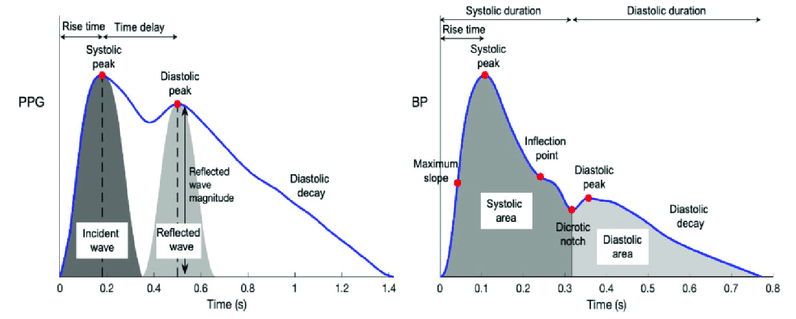
\includegraphics[width=\textwidth]{images/sp/pwa}
    \caption{Example of a PWA used to extract features from the PPG waveform~\cite{bikiaLeveragingPotentialMachine2021}}
    \label{fig:pwa}
\end{figure}

% Different types of filters for processing the PPG signal
\vspace{0.2cm}
\textit{Signal Pre-Processing}
\vspace{0.2cm}

The preprocessing of physiological signals, crucial for accurate BP estimation, involves a variety of signal filtering techniques.
Techniques like Chebyshev, Butterworth, and Savitzky-Golay filtering, along with methods such as second derivative analysis, play pivotal roles in enhancing signal quality.
These preprocessing steps, facilitated by advancements in computational technology, pave the way for more refined analysis and interpretation of PPG pulse waves.

% Butterworth
An investigation into various signal pre-processing techniques necessitates an examination of different types of filters.
One prominent representative is the Butterworth filter, characterized by its flat frequency response within the passband.
Belonging to the Infinite Impulse Response (IIR) category, Butterworth filters offer efficiency in processing low-frequency signals and exhibit rapid computational capabilities, as demonstrated by Chatterjee et al.\ in their PPG-based heart rate analysis~\cite{chatterjeePPGBasedHeart2018}.
The filter order directly correlates with the number of energy storage components present in the analogous analog circuit, such as inductors and capacitors.
The transfer function of a Butterworth filter is represented by the following formula, where \texttt{n} is the filter order and \texttt{z} is the complex variable used in Z-transform analysis:
\Large
\begin{center}
    \begin{math}
        H(z) = \frac{1}{[1 + (z^{-1})^{n}]^{1/2}}
    \end{math}
\end{center}
\normalsize

% SavGol
Another noteworthy filter type is the Savitzky-Golay filter, introduced by Savitzky and Golay~\cite{savitzkySmoothingDifferentiationData1964}.
Falling under the Finite Impulse Response (FIR) category, this filter effectively smooths data while removing unwanted frequencies.
Its inherent stability ensures a finite output for any finite input.
Additionally, the linear phase property guarantees the absence of frequency-dependent time shifts.
The Savitzky-Golay filter doesn't have a single transfer function like the Butterworth filter because it belongs to the FIR category.
Instead, it relies on convolution with pre-calculated coefficients specific to the desired characteristics.
The filter fits a low-degree polynomial to a window of data points around each point in the signal.
The smoothed value is then the value of the fitted polynomial at the center point.
Different polynomial degrees and window sizes lead to different filtering effects.
The relationship can be expressed by the following formula:
%\Large
%\begin{center}
%    \begin{math}
%        y[n]~=~\sum_{i=-\frac{M}{2}}^{\frac{M}{2}} W_i~\cdot~x_{n+i} \\
%        \normalsize
%        \begin{array}{ll}
%            M       & : \text{Window size (odd number greater than or equal to N+1)} \\
%            N       & : \text{Polynomial degree}                                     \\
%            W_i     & : \text{Filter coefficients (length M)}                        \\
%            x_{n+i} & : \text{Signal data point}                                     \\
%            y[n]    & : \text{Smoothed data point}
%        \end{array}
%    \end{math}
%\end{center}
%\normalsize

% Chebyshev
Furthermore, the Chebyshev filter offers a steeper roll-off compared to other filters, leading to sharper distinctions between desired and unwanted frequencies.
While this advantage comes at the cost of controlled passband ripples, these filters remain valuable tools for applications requiring precise frequency separation.
Beyond digital signal improvement, they find applications in audio crossovers, image noise reduction, and data communication, as discussed by Antoniou~\cite{antoniouDigitalFiltersAnalysis2018}.
While the Chebyshev filter has a transfer function like the Butterworth filter, it's slightly more complex due to its specific characteristics.
Unlike the Savitzky-Golay filter, its coefficients depend on the desired ripple level and order, making a single, universal formula impractical.
The general form of the Chebyshev filter transfer function depends on whether it's Type I (equiripple in both passband and stopband) or Type II (equiripple only in the stopband).
The corresponding functions are presented by the following formulas:~
%\begin{multicols}{2}
%    \begin{center}
%        Chebyshev I \\
%        \vspace{0.2cm}
%        \large
%        \begin{math}
%            H(z) = K \prod_{n=1}^{N} \left[ 1 - \frac{\varepsilon}{(T_n(z))^2} \right]
%        \end{math}
%        \normalsize
%        \begin{tabular}{ll}
%            $K$           & : Gain factor                 \\
%            $\varepsilon$ & : Normalized passband         \\           & \;\, ripple level (dB)                \\
%            $N$      & : Filter order \\
%            $T_n(z)$      & : Chebyshev polynomial of the \\      & \;\, first kind, evaluated at $z$ \\
%        \end{tabular}
%    \end{center}
%    \columnbreak
%    \begin{center}
%        Chebyshev II \\
%        \vspace{0.2cm}
%        \large
%        \begin{math}
%            H(z) = K \cdot \frac{z^N - 1}{\prod_{n=1}^{N} \left[ z^2 - 2 \zeta z \cos(\omega_n) + 1 \right]}
%        \end{math}
%        \normalsize
%        \begin{tabular}{ll}
%            $K$        & : Gain factor                        \\
%            $N$        & : Filter order                       \\
%            $\zeta$    & : Normalized stopband damping factor \\
%            $\omega_n$ & : Normalized cutoff frequency        \\
%        \end{tabular}
%    \end{center}
%\end{multicols}

% Optimal finding
In their 2018 study, Liang et al.\ investigated nine different digital signal filters to identify the optimal approach for short PPG signals (2.1s)~\cite{liangOptimalFilterShort2018}.
Some of the filters included the Butterworth, Elliptical, Chebyshev Type I and II, Median Filter etc.
Their performance-based ranking revealed the Chebyshev II filter as the most effective in enhancing PPG signal quality, with the optimal order at 4th.

% miscallaneous sp approaches
\vspace{0.2cm}
\textit{Miscellaneous Signal Processing Approaches}
\vspace{0.2cm}

A study conducted by Takazawa et al.\ investigated the utilization of the second derivative of the fingertip PPG waveform within clinical contexts~\cite{takazawaAssessmentVasoactiveAgents1998}.
The research analysed changes in patients' pressure, wave ratios, age-related variations, and correlations with health conditions.
Collectively, the results indicate the potential value of the second derivative in appraising the impacts of specific medications and assessing vascular health and aging, offering potential avenues in arteriosclerotic disease screening.
Subsequent research has demonstrated the effective application of the second derivative of the PPG waveform in identifying the dicrotic notch within a single pulse wave (see Figure~\ref{fig:dic_notch}), a critical landmark in PWA\@.

\begin{figure}[h]
    \centering
    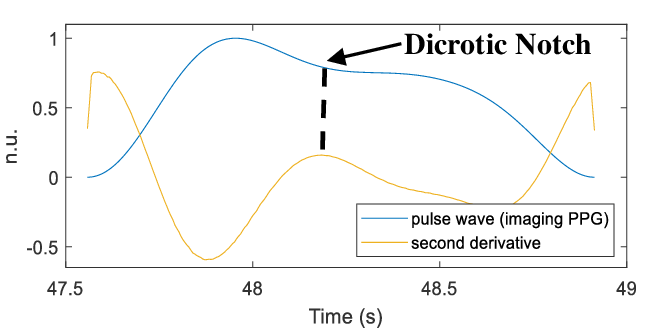
\includegraphics[scale=0.6]{images/sp/dic_notch}
    \caption{Dicrotic Notch Approximation from the Second Derivate of the PPG~\cite{djeldjliImagingPhotoplethysmographySignal2019}}
    \label{fig:dic_notch}
\end{figure}

In 2022, Charlton et al.\ conducted a collaborative study to investigate the hemodynamic characteristics of photoplethysmogram (PPG) waveforms for the purpose of vascular age assessment~\cite{charltonAssessingHemodynamicsPhotoplethysmogram2022}. A key outcome of their work was the identification of a comprehensive set of features, termed "fiducial points," which could be extracted from the PPG waveform to achieve accurate vascular age estimation.

The term \enquote{fiducial} originates from the Latin \textit{fiducialis}, meaning \enquote{reliable}.
In the context of signal processing, it refers to reference points employed for precise measurements.
In the early cases, it has been used for accurate determination of pulse transit time (PTT) between the R-wave of the electrocardiogram (ECG) and a designated point in a finger PPG pulse, as demonstrated by Zhang et al.~\cite{zhangEffectLocalCold2005}.
In the study by Charlton et al., these points were repurposed to delineate diverse landmarks (identified as Row A in Figure~\ref{fig:fiducials}) on the pulse wave, serving as references for extracting both temporal and amplitude-based features.

\begin{figure}[h]
    \centering
    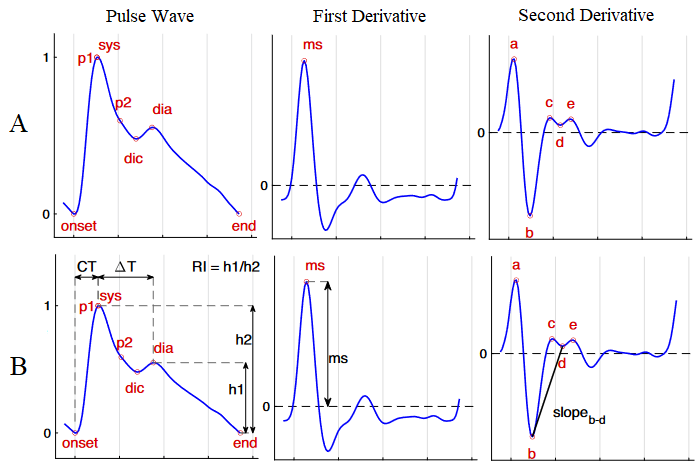
\includegraphics[scale=0.8]{images/sp/fiducials}
    \caption{A - Fiducial Point Identification; B - Feature Calculation~\cite{charltonAssessingHemodynamicsPhotoplethysmogram2022}}
    \label{fig:fiducials}
\end{figure}

Building upon the identified fiducial points, Charlton et al.\ employed various techniques to extract meaningful values from a single PPG signal (Row B in Figure~\ref{fig:fiducials}) that contribute to vascular age assessment.
This section provides a summary of the implemented methods and corresponding example values (presented in brackets):
\begin{enumerate}
    \item Pulse Wave Features (crest time: time from \texttt{onset} to \texttt{sys})
    \item First Derivative Features (minimum rise time: amplitude of pulse wave divided by amplitude of \texttt{ms})
    \item Second Derivative Features (aging index: defined as amplitude values of \mbox{\texttt{(b-c-d-e)/a)}}
    \item Combination of Features (minimum rise time: \texttt{[1/x0(ms)]·[x(sys) - x(onset)]})
    \item Frequency Domain Analysis (Fast Fourier Transform (FFT) analysis: Use of FFT to extract amplitude and phase information from the PPG signal)
    \item Features From Multiple Beats (pulse rate variability parameters)
\end{enumerate}

\vspace{0.2cm}
This section explored diverse signal processing techniques.
As mentioned previously, traditional methods relying on physiological parameters (PAT, PTT, PWV) face limitations.
Signal processing approaches like PWA, filtering, and feature extraction are often integrated with ML models and provide a higher BP detection accuracy.
These approaches show promising results for cuffless, continuous BP estimation using PPG signals, paving the way for practical non-invasive BP monitoring solutions.

\subsubsection{Machine Learning}
\label{subsubsec:machine_learning}

Building upon the foundation laid by traditional signal processing techniques, ML emerges as a transformative force in the pursuit of accurate and non-invasive BP estimation using PPG signals.
This section delves into the diverse tapestry of ML methods currently employed, thoroughly exploring their individual approaches and their collective potential to improve cuffless BP monitoring.

\begin{figure}[h]
    \centering
    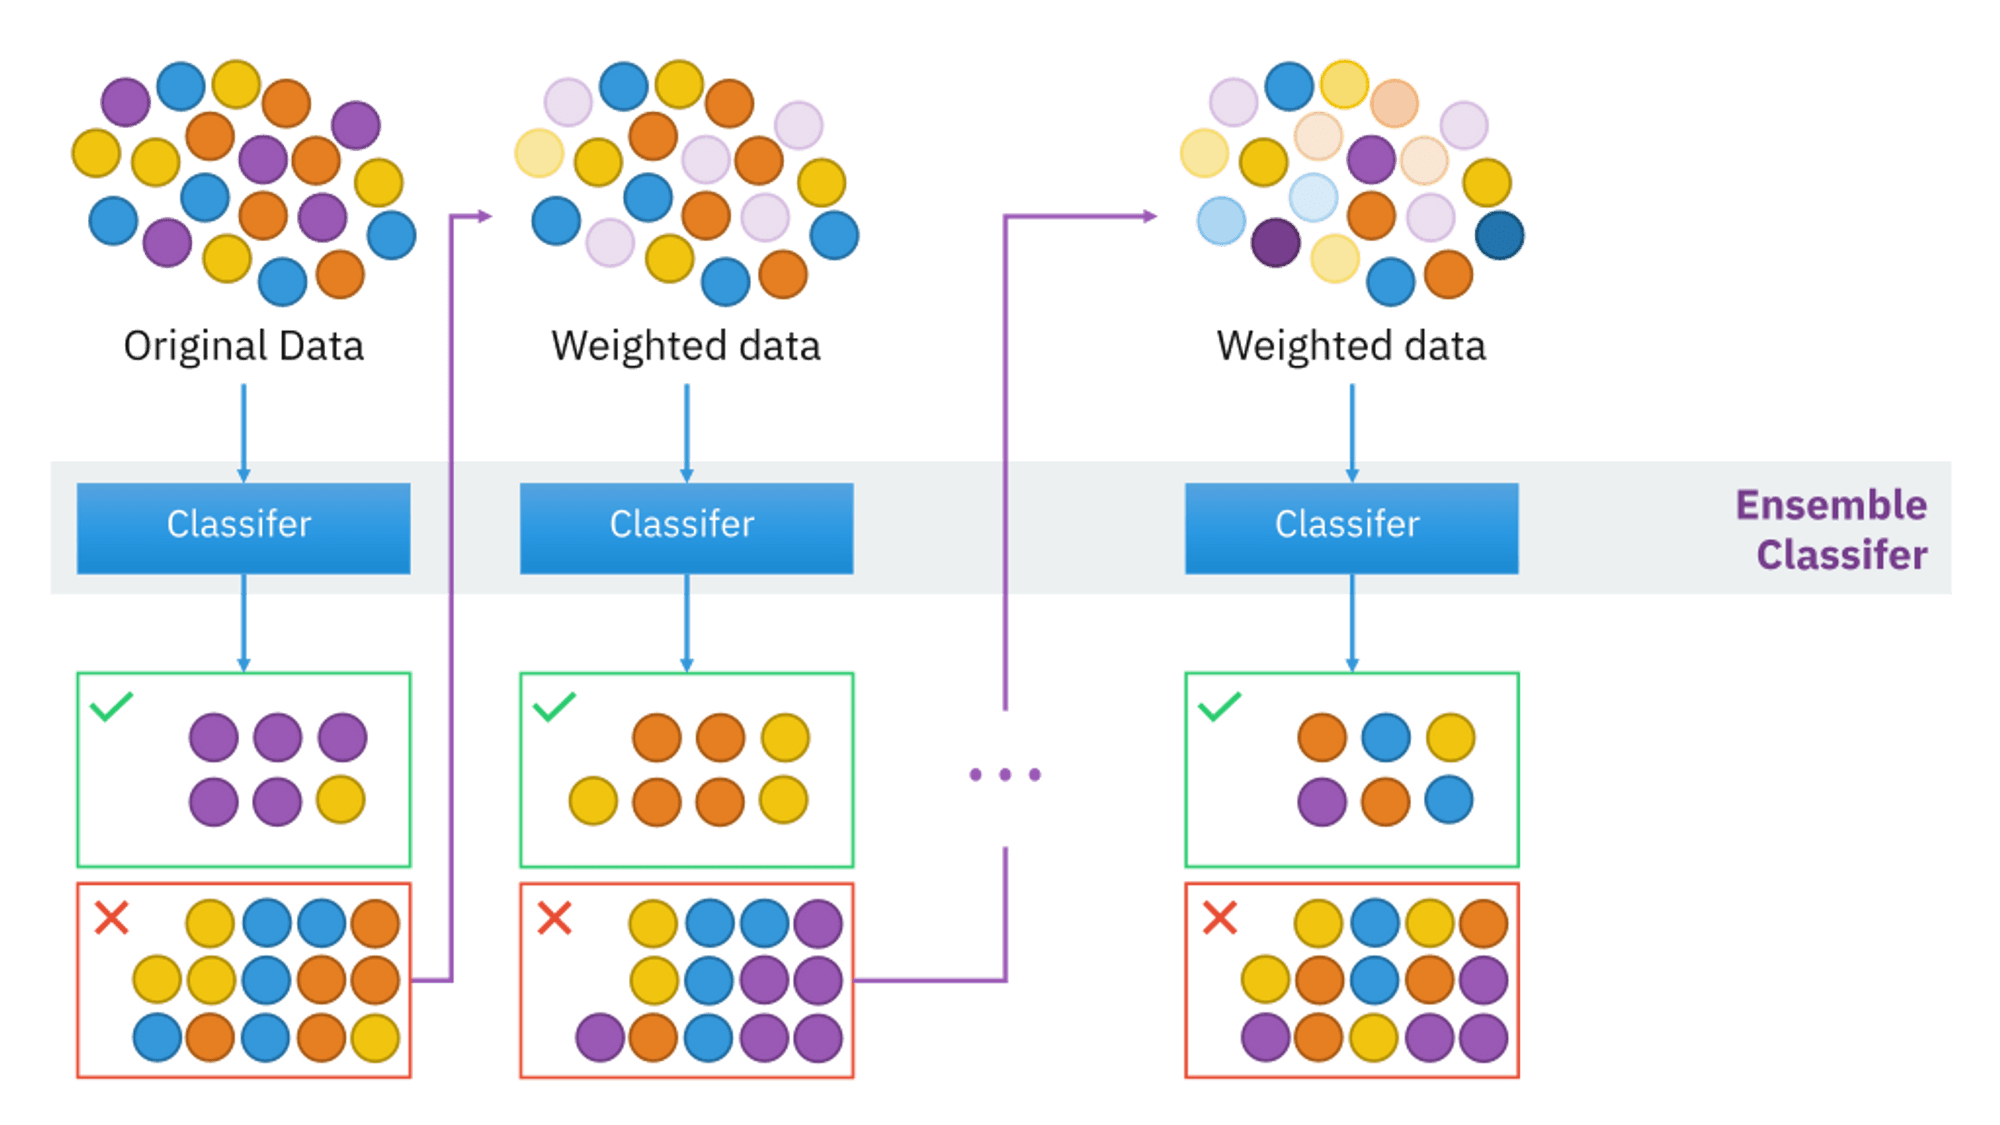
\includegraphics[scale=0.06]{images/ml/adaboost}
    \caption{\small AdaBoost, or Adaptive Boosting, is an ensemble learning technique that iteratively combines weak classifiers to create a strong classifier by adjusting weights based on classification errors~\cite{AdaBoostAlgorithmMachine}}
    \label{fig:adaboost}
\end{figure}

% ML Techniques
\vspace{0.2cm}
\textit{Machine Learning Approaches}
\vspace{0.2cm}

BP estimation using ML techniques is data driven, unlike the traditional PTT/PAT only models.
Several studies attempted to fit regression models, such as multilinear regression, support vector machine (SVM) and random forest, for estimating BP using PTT/PAT based approach with some degree of success, but the results did not always satisfy the international standards.

As early as 2003, Teng and Zhang~\cite{tengContinuousNoninvasiveEstimation2003} were among the pioneers in exploring non-invasive methods for estimating blood pressure without the need for traditional cuff-based techniques.
They explored the relationship between four PPG features and BP using a linear regression (LR) model.
While diastolic time exhibited the strongest correlation with both SBP and DBP, the overall results suggested limitations in LR for accurate BP estimation.

Recognizing these limitations, Suzuki and Oguri (2009) introduced AdaBoost (example in Figure~\ref{fig:adaboost}), a classifier, for SBP estimation~\cite{suzukiCufflessBloodPressure2009}.
This methodology segmented SBP values using a threshold before employing a nonlinear ML model, showcasing the need for more complex techniques.

Seeking a different approach, Ruiz-Rodriguez et al.\ (2013) utilized a Deep Belief Network Restricted Boltzmann Machine (RBM) for simultaneous prediction of SBP, DBP, and MAP~\cite{ruiz-rodriguezInnovativeContinuousNoninvasive2013a}.
An example DBN and RBM with custom input and output sizes is illustrated in Figure~\ref{fig:rbm}
However, the study yielded highly variable results, raising concerns about its reliability.

\begin{figure}[h]
    \centering
    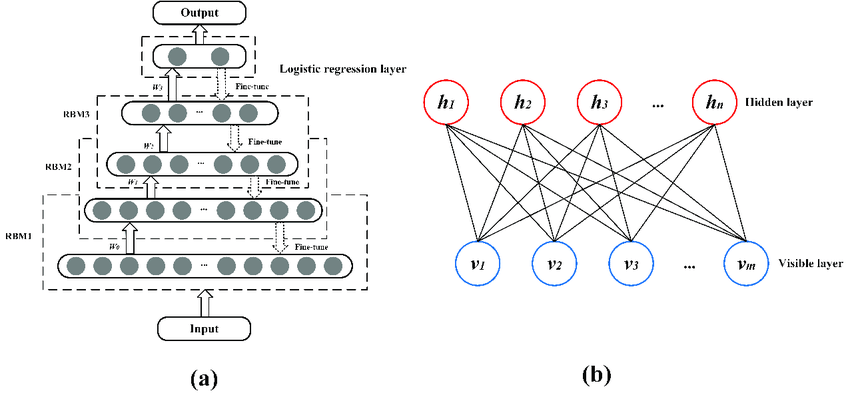
\includegraphics[scale=0.5]{images/ml/RBM}
    \caption{\small A DBN (a) combines multiple layers of RBMs (b) to form a generative model capable of learning hierarchical representations of the data~\cite{ouIntegratingCellularAutomata2019}}
    \label{fig:rbm}
\end{figure}

Shifting focus to feature extraction, Kurylyak et al.\ (2013) extracted 21 features from the PPG waveform and used a feedforward NN (example in Figure~\ref{fig:ffnn}) for SBP and DBP estimation~\cite{kurylyakNeuralNetworkbasedMethod2013}.
Their promising results demonstrated the potential of NN-based approaches.

\begin{figure}[h]
    \centering
    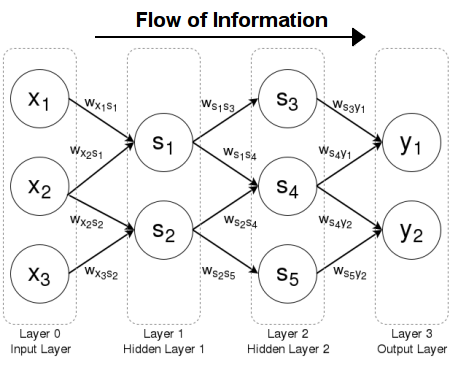
\includegraphics[scale=0.5]{images/ml/ffnn}
    \caption{\small Feed Forward NNs have connections between the nodes that do not form cycles, allowing data to move in only one direction, from the input nodes through the hidden nodes to the output nodes, with each connection having an associated weight~\cite{FeedforwardNeuralNetworks}}.
    \label{fig:ffnn}
\end{figure}

Xing and Sun (2016) ventured into the frequency domain, applying Fast Fourier Transformation to select features followed by a feedforward NN for BP estimation~\cite{xingOpticalBloodPressure2016}.
While initial results were encouraging, the authors recognized the need for broader feature space exploration.

Building upon Kurylyak et al.'s work, Liu et al.\ (2017) incorporated 14 second derivative features and employed an SVM for BP estimation, highlighting the value of diverse feature extraction techniques~\cite{liuIntegratedNavigationTethered2017}.

Marking a significant shift, Su et al.\ (2018) explored a four-layer bidirectional Long Short-term memory (LSTM) model with residual connections, demonstrating the promise of recurrent NNs~\cite{suLongtermBloodPressure2018}.
The working principle of an LSTM is demonstrated in Figure~\ref{fig:lstm}.

\begin{figure}[h]
    \centering
    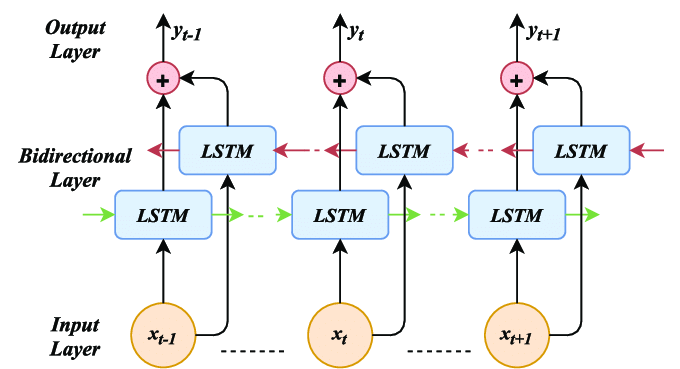
\includegraphics[scale=0.5]{images/ml/lstm}
    \caption{\small Bidirectional LSTM is a type of recurrent neural network architecture that processes sequential data in both forward and backward directions. This allows the model to capture dependencies from past and future contexts simultaneously, enhancing its ability to understand and predict patterns in sequential data~\cite{anishnamaUnderstandingBidirectionalLSTM2023}}.
    \label{fig:lstm}
\end{figure}

A 2019 study by Tanveer and Hasan introduced a hierarchical Artificial NN-LSTM model for blood pressure estimation, comprising two levels: the lower level employed ANNs to extract morphological features from ECG and PPG waveforms, while the upper level utilized LSTM layers to address temporal variations in these features~\cite{tanveerCufflessBloodPressure2019}.
They also found, that DBP is strongly associated with SBP and can enhance its estimation, suggesting simultaneous modeling using a single architecture for both.

Focusing on long term estimation, El-Hajj and Kyriacou (2021) proposed leveraging advanced deep learning techniques like Bidirectional-LSTMs and Bidirectional Gated Recurrent Units (GRU) with attention mechanisms (example of attention mechanism implementation in LSTM in Figure~\ref{fig:attention}) for BP estimation~\cite{el-hajjDeepLearningModels2021}.

\begin{figure}
    \begin{minipage}[c]{0.5\textwidth}
        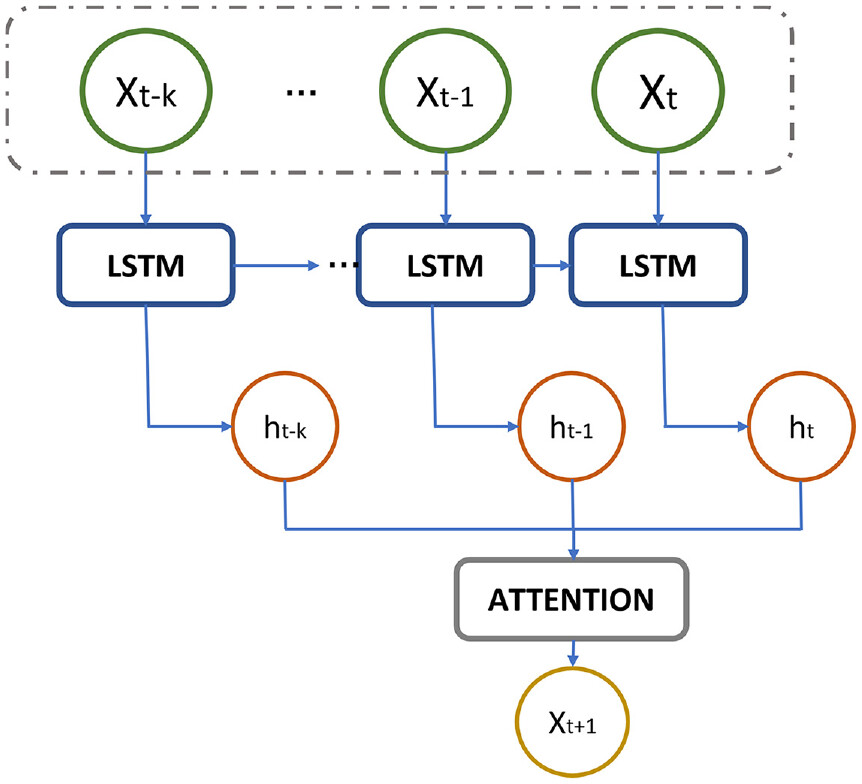
\includegraphics[width=\textwidth]{images/ml/attention}
    \end{minipage}\hfill
    \begin{minipage}[c]{0.5\textwidth}
        \captionsetup{format=plain, justification=centering}
        \caption{\small The attention mechanism in LSTM allows the model to focus on specific parts of the input sequence, dynamically adjusting the importance of each input element during the prediction process~\cite{marulandaHybridModelBased2023}}
        \label{fig:attention}
    \end{minipage}
\end{figure}

%\begin{figure}
%\floatbox[{\capbeside\thisfloatsetup{capbesideposition={right,top},capbesidewidth=4cm}}]{figure}[\FBwidth]
%{\caption{A test figure with its caption side by side}\label{fig:at}}
%{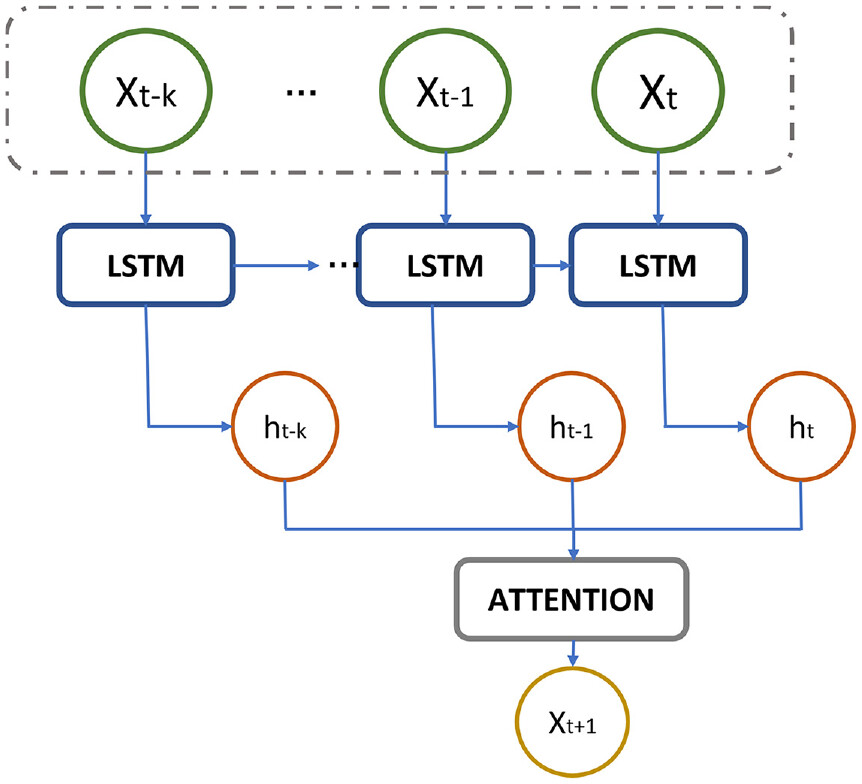
\includegraphics[scale=0.5]{images/ml/attention}}
%\end{figure}

Recognizing the need for real-world applicability, Joung et al.\ (2023) evaluated a learning-driven cuffless BP estimation system under challenging conditions with calibration~\cite{joungContinuousCufflessBlood2023}.
Their 1D convolutional NN highlighted the importance of addressing various real-world scenarios.

These early studies illustrate the evolution of ML techniques for cuffless BP estimation, paving the way for further advancements.
From exploring linear relationships to harnessing the power of deep learning, researchers continue to refine and develop novel approaches.
While challenges remain, these pioneering efforts demonstrate the immense potential of ML in improving non-invasive BP monitoring, and future research holds the promise for even more accurate and robust solutions.

\vspace{0.2cm}

To conclude, the relationship between PPG characteristics and BP was not found to consistently follow a linear trend.
Conventional linear models frequently struggle to effectively capture the complex relationship between BP and PPG when analysed across various demographic datasets.
Traditional ML algorithms like SVMs and Random Forest tend to achieve higher accuracy rates in this context.
To estimate BP accurately using these techniques, distinct models are typically constructed for SBP and DBP\@.
However, recent evidence suggests that a unified architecture capable of simultaneously modeling SBP, DBP, and even MAP is both feasible and advantageous.
Various advanced NN models demonstrate superior efficiency in integrating such architectures and leveraging extensive datasets with heightened precision relative to conventional ML approaches.

\section{Methods}
\label{sec:methods}

\begin{enumerate}

\item Data fetching and reading using WFDB and NumPy libraries.

\item Digital signal filtering using Savitzky-Golay and Butterworth Lowpass filters.

\item Beat detection algorithms from MIMIC WFDB Tutorial used for primary estimation.
Beat detection improved with manual implementation of SciPy library.

\item Fiducial Point calculation based on the algorithm provided in the MIMIC WFDB Tutorial.

\item Feature extraction with personally created code to extract time domain features, and NumPy library to extract frequency domain features (FFT). Median value calculation using NumPy library.

\item Machine Learning Model creation using PyTorch and Scikit-Learn libraries.

\end{enumerate}

\section{Results}
\label{sec:results}

\subsection{Data Fetching}
\label{subsec:data_fetching}

Data for Validation from MIMIC4:
5508 records each containing 37795 values corresponding to ~605 seconds (fs=64.4725);

Data for Training/Testing from MIMIC3 (1st Iteration):
306 records each containing 75625 values corresponding to 605 seconds (fs=125);

\subsection{Data Processing}
\label{subsec:data_processing}

Same Signaling processing approaches were included (see 4.2) for both the MIMIC4 and MIMIC3 data.

\subsection{Feature Extraction}
\label{subsec:feature_extraction}

CAVE: out of the 34 features, 2 (delta T and resistive index) depend on the accurate detection of the dicrotic notch.
Significantly more values can be extracted if finding the dicrotic notch would not be necessary

FE from MIMIC4:
- For target reference Systolic, Diastolic and MAP values were extracted from the waveform data.
- For Machine Learning, 34 features were extracted from the PPG waveform
A total of n values were extracted, resulting in a 34 x n matrix.
Total of m median values were extracted

FE 1st iteration from MIMIC3:

- For target reference ABP Systolic and Diastolic values were extracted from the waveform data.
- For Machine Learning, 34 features were extracted from the PPG waveform
A total of 161,269 values were extracted, resulting in a 34x161269 matrix.
Total of 14,958 median values were extracted

\subsection{Machine Learning}
\label{subsec:machine_learning}

\section{Discussion}
\label{sec:discussion}

Limitations:
- not knowing what devices were used
- how they were calibrated
- how accurate they are
- pulse oximeter and arterial catheter parameters
- sampling rates are different for every device (even between MIMIC 3 and 4)

Possible Improvements:
- integrate both the ECG and PPG graphs for a more precise prediction
- use further signal processing approaches
- manually filter waveform graphics (e.g.\ faulty PPG signal)
- expand on machine learning algorithms

\section{Conclusion}
\label{sec:conclusion}

\bibliographystyle{plain}
\bibliography{literature}

\end{document}